\documentclass[useAMS, usenatbib, a4paper]{mnras}
\pdfsuppresswarningpagegroup=1

\usepackage{graphicx}
\usepackage{microtype}
\usepackage{xcolor}
\usepackage{fixltx2e}
\usepackage{booktabs}
\usepackage{siunitx}
\sisetup{separate-uncertainty = true}
\usepackage{color}
\usepackage{enumerate}
\usepackage{pdflscape}
\usepackage{rotating}
\usepackage{xr-hyper}
\usepackage{hyperref}
\externaldocument[Q-]{quadrics-bowshock}

\usepackage[T1]{fontenc} 
\usepackage[utf8]{inputenc}

% Fonts 
\usepackage{newtxtext}
% Note: newtxmath must come AFTER newtxtext
\usepackage[varvw,smallerops]{newtxmath}

\usepackage{chemgreek}
\activatechemgreekmapping{newtx}

\hypersetup{colorlinks=True, linkcolor=blue!50!black, citecolor=black,
  urlcolor=blue!50!black}

\usepackage{etoolbox}
\robustify\bfseries
\robustify\itshape

%% The following hack solves a problem with
%% ERROR: \pdfendlink ended up in different nesting level than \pdfstartlink.
%% See https://tex.stackexchange.com/a/249743
\makeatletter
\patchcmd\@combinedblfloats{\box\@outputbox}{\unvbox\@outputbox}{}{%
  \errmessage{\noexpand\@combinedblfloats could not be patched}%
}%
\makeatother

%% Bold italic
\newcommand\hmmax{0}            % we don't need heavy fonts
\newcommand\bmmax{1}            % reduce use of math alphabets for bold
\usepackage{bm}

%% Bundled custom packages
\usepackage{aastex-compat}

\title
% {No radiation supported dust wave around \(\sigma\) Orionis}
% OR
% {\boldmath A dusty bow shock around \(\sigma\) Orionis driven by an enclosed proplyd?}
% OR
{\boldmath Bow shocks, bow waves, and dust waves. V. No dust wave for \(\sigma\) Ori}


\newcommand\AddressCRyA{Instituto de Radioastronom\'{\i}a y Astrof\'{\i}sica,
  Universidad Nacional Aut\'onoma de M\'exico, Apartado Postal 3-72,
  58090 Morelia, Michoac\'an, M\'exico}
\author[Henney \& Arthur]{
  William J. Henney \& S. Jane Arthur\\
  \AddressCRyA
}

% These dates will be filled out by the publisher
\date{Accepted XXX. Received YYY; in original form ZZZ}

% Enter the current year, for the copyright statements etc.
\pubyear{2017}
\DeclareMathOperator{\sgn}{sgn}
\DeclareMathOperator{\Sin}{\mathcal{S}}
\DeclareMathOperator{\Cos}{\mathcal{C}}
\DeclareMathOperator{\Cot}{\mathcal{T}}
\DeclareMathOperator{\GammaFunc}{\Gamma}
\newcommand\w{\ensuremath{\mathrm{w}}}
\newcommand\C{\ensuremath{\mathrm{c}}}
\providecommand{\abs}[1]{\lvert#1\rvert}
\providecommand{\Abs}[1]{\left\lvert#1\right\rvert}
\newcommand\TODO[1]{%
  \begin{center}
    \framebox{\parbox{0.8\linewidth}{
        \texttt{\footnotesize\color{red} #1}}}
  \end{center}}

\newcommand\uvec[1]{\bm{\hat{#1}}}
\newcommand\T{_{\mathrm{\scriptscriptstyle T}}}

\newcommand\Qp{\ensuremath{Q_{\text{p}}}}
\newcommand{\grain}{\ensuremath{_{\text{d}}}}
\newcommand{\B}{\ensuremath{_{\scriptscriptstyle\text{B}}}}
\newcommand{\alfven}{\ensuremath{_{\scriptscriptstyle\text{A}}}}
\newcommand{\xsec}{\ensuremath{\sigma\grain}}
\newcommand\frad{\ensuremath{f_{\text{rad}}}}
\newcommand\fmax{\ensuremath{f_{\text{max}}}}
\newcommand\thm{\ensuremath{\theta_{\text{m}}}}
\newcommand\drag{\ensuremath{_{\text{drag}}}}
\newcommand{\gas}{\ensuremath{_{\text{gas}}}}
\newcommand{\drift}{\ensuremath{_{\text{drift}}}}
\newcommand\rad{\ensuremath{_{\text{rad}}}}
\newcommand\Rmin{\ensuremath{R_{\scriptscriptstyle\text{min}}}}
% Why do I need both of these?
\newcommand\sound{\ensuremath{c_{\text{s}}}}
\newcommand\soundspeed{\ensuremath{c_{\text{s,gas}}}}
\newcommand\starstar{\ensuremath{_{**}}}
\newcommand\hii{\ion{H}{ii}}


\defcitealias{Tarango-Yong:2018a}{Paper~I}
\newcommand\PaperI{\citetalias{Tarango-Yong:2018a}}


\begin{document}
\label{firstpage}
\pagerange{\pageref{firstpage}--\pageref{lastpage}}
\maketitle
\begin{abstract}
  We critically evaluate the role of radiation and ram pressure in
  providing internal support for the bow-shaped infrared arc around
  the massive triple star system \(\sigma\)~Ori Aa/Ab/B in the IC434 \hii{}
  region.  We present evidence for hydrogen recombination line
  emission from the arc, which demonstrates that it cannot be a
  decoupled dust wave, as has previously been claimed.  On the other
  hand, we show that the fraction of the stellar luminosity trapped by
  the arc is insufficient for it to be supported by radiation if the
  grains and gas are well coupled.  Therefore, the arc must be
  supported by the ram pressure of an internal wind.  However, the
  stellar winds from the OB stars in the \(\sigma\)~Ori Aa/Ab/B system seem
  too weak to provide this support on their own.  We propose instead
  that it is the photoevaporated disk wind from the enclosed proplyd
  IRS~1B that dominates the ram pressure support for the bow.
\end{abstract}

\begin{keywords}
  circumstellar matter -- radiation: dynamics -- stars: winds, outflows
\end{keywords}

\section{Why the inner arc cannot be a decoupled dust wave}
\label{sec:why-not-dust}

We downloaded optical images of \(\sigma\)~Ori from the Astronomical Data
Centre of the Cambridge Astronomy Survey
Unit.\footnote{\url{http://casu.ast.cam.ac.uk/surveys-projects/adc}}
These were obtained on 2008-11-19 with the Wide Field Camera of the
Isaac Newton Telescope from an observational program of Rafael
Barrena.  We use images in two filters: a narrow-band H\(\alpha\) filter
(central wavelength, \(\lambda_0 = \SI{656.8}{nm}\), full-width half
maximum, \(\Delta\lambda = \SI{9.5}{nm}\)) and a broad-band Sloan Gunn
\(R\) filter (\(\lambda_0 = \SI{624.0}{nm}\), \(\Delta\lambda = \SI{134.7}{nm}\)).  We have removed the bias v

\section{Why the inner arc cannot be radiation-supported}
\label{sec:why-not-radiation}

SEDs of the two arcs

\begin{figure}
  \centering
  \includegraphics[width=\linewidth]{figs/sigma-ori-comparison}
  \caption{Optical and infrared images of $\sigma$~Ori and its
    surroundings.  (a)~Optical image in in the H\(\alpha\) line, shown in
    negative grayscale.  (b)~Mid-infrared image in three Spitzer
    bands: MIPS \SI{23.7}{\um} (red), IRAC \SI{7.87}{\um} (green), and
    IRAC \SI{5.73}{\um} (blue).  The yellow dashed box shows the slit
    for which profiles are extracted in Fig.~\ref{fig:sig-ori-cuts}.}
  \label{fig:sig-ori}
\end{figure}

\begin{figure}
  \centering
  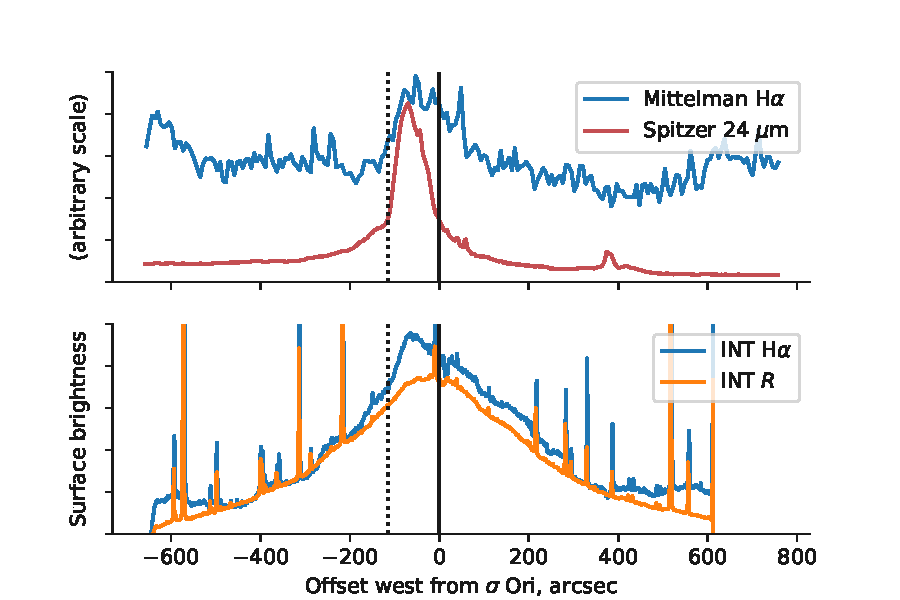
\includegraphics[width=\linewidth]{figs/sigma-ori-eastwest-cuts}
  \caption{Brightness profiles through $\sigma$~Ori inner arc.  (a)~H\(\alpha\) and  All
    profiles are extracted in a \(40''\) wide slit, offset by \(80''\)
    to the south of \(\sigma\)~Ori, as indicated in
    Fig.~\ref{fig:sig-ori}b. }
  \label{fig:sig-ori-cuts}
\end{figure}

\begin{figure}
  \centering
  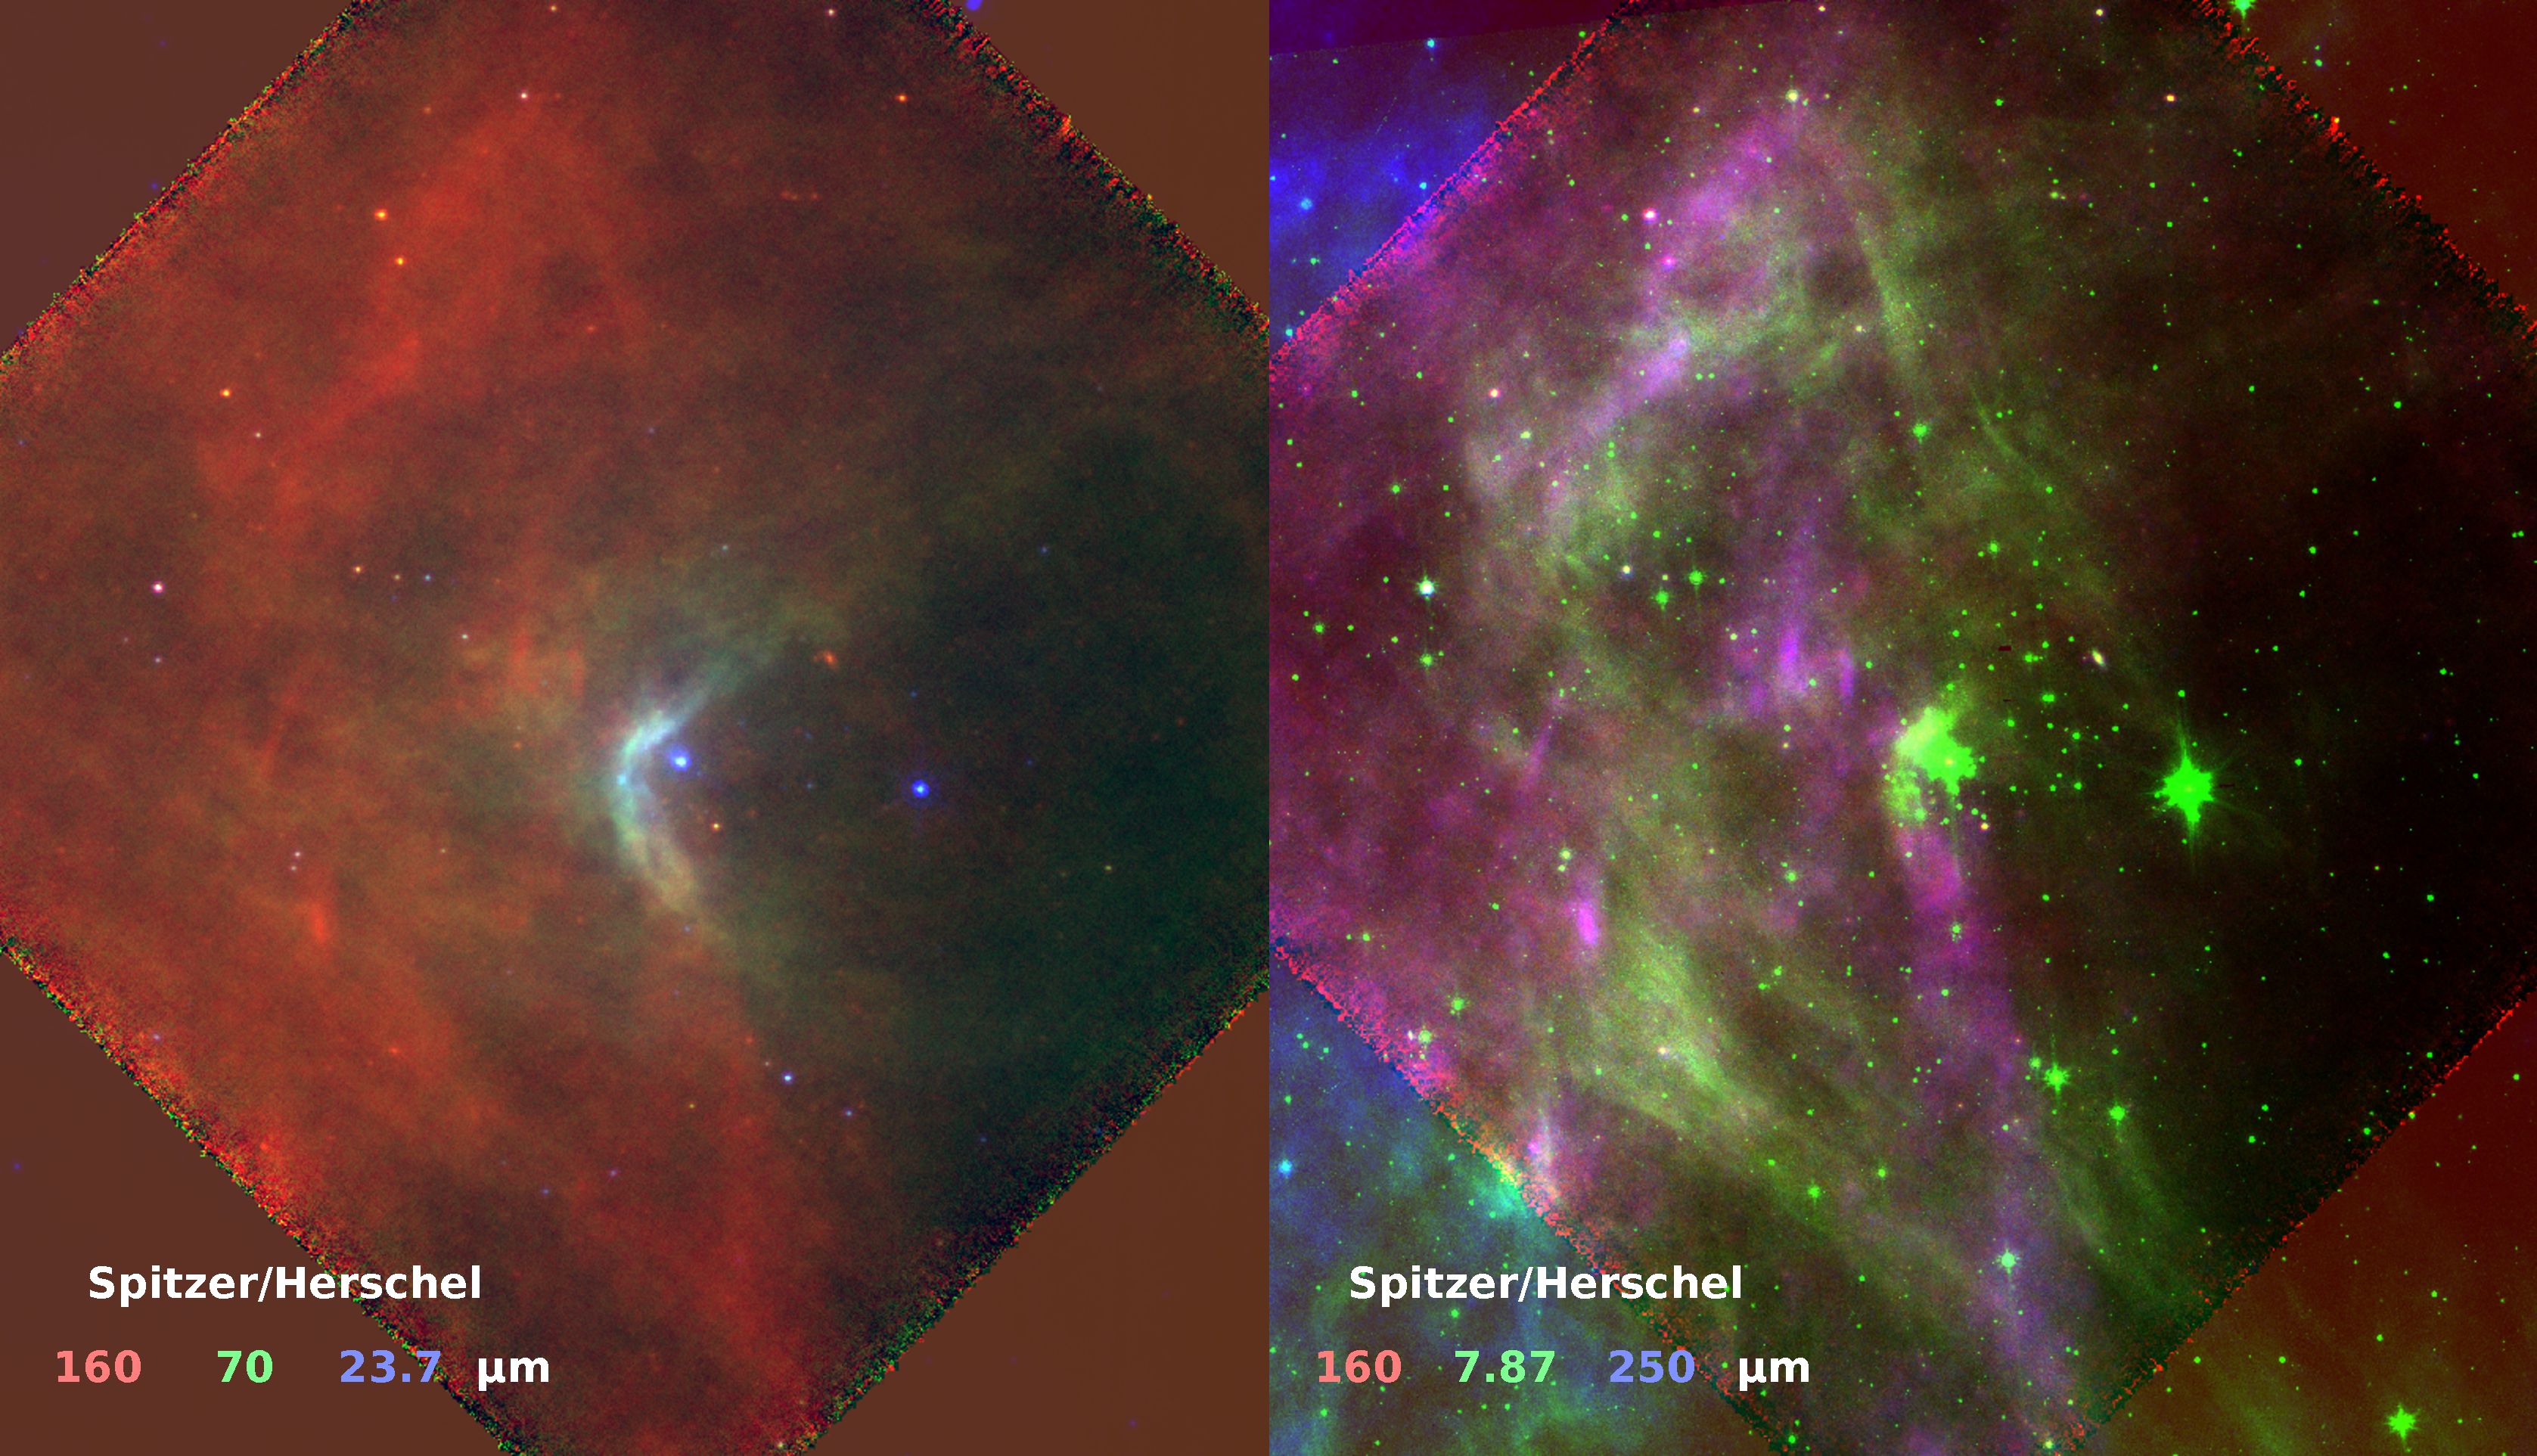
\includegraphics[width=\linewidth]{figs/sigma-ori-inner-outer}
  \caption{Combined mid-infrared and far-infrared views of the inner
    and outer arcs around $\sigma$~Ori}
  \label{fig:sig-ori-outer}
\end{figure}

\begin{figure}
  \centering
  \caption{Spectral energy distributions of arcs around $\sigma$~Ori}
  \label{fig:sig-ori-SED}
\end{figure}



\section{Weak stellar winds from the massive triple Aa/Ab/B}
\label{sec:stellar-winds-AB}

\section{Photoevaporation flow from the proplyd IRS~1B}
\label{sec:phot-flow-from}

\section{The nature of the outer dust arc}

\begin{figure}
  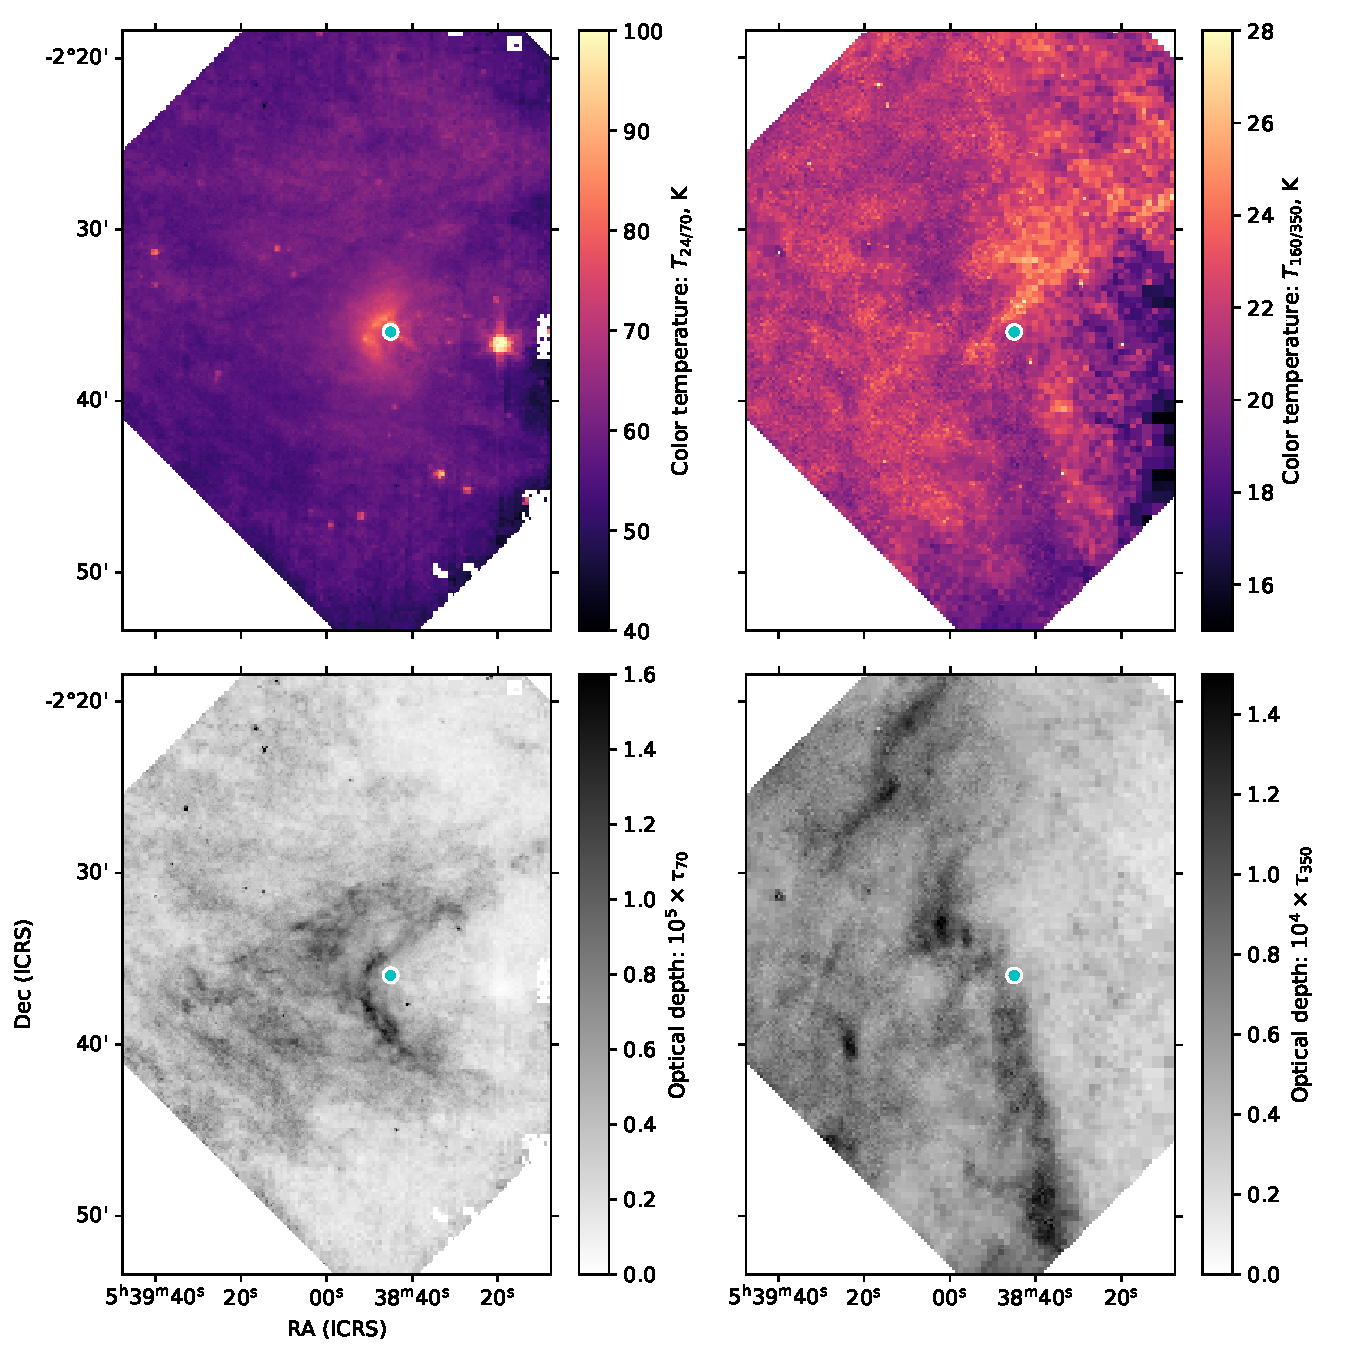
\includegraphics[width=\linewidth]{figs/sigma-ori-multi-Tcol-tau}
  \caption{Maps of dust temperature and optical depth. (a)~Color
    temperature derived from \(\SI{24}{\um} /
    \SI{70}{\um}\). (b)~Color temperature derived from
    \(\SI{160}{\um} / \SI{350}{\um}\). (c)~\SI{70}{\um} optical depth
    of warm dust component. (d)~\SI{350}{\um} optical depth of cool
    dust component.}
  \label{fig:N-T-distro}
\end{figure}


\begin{figure}
  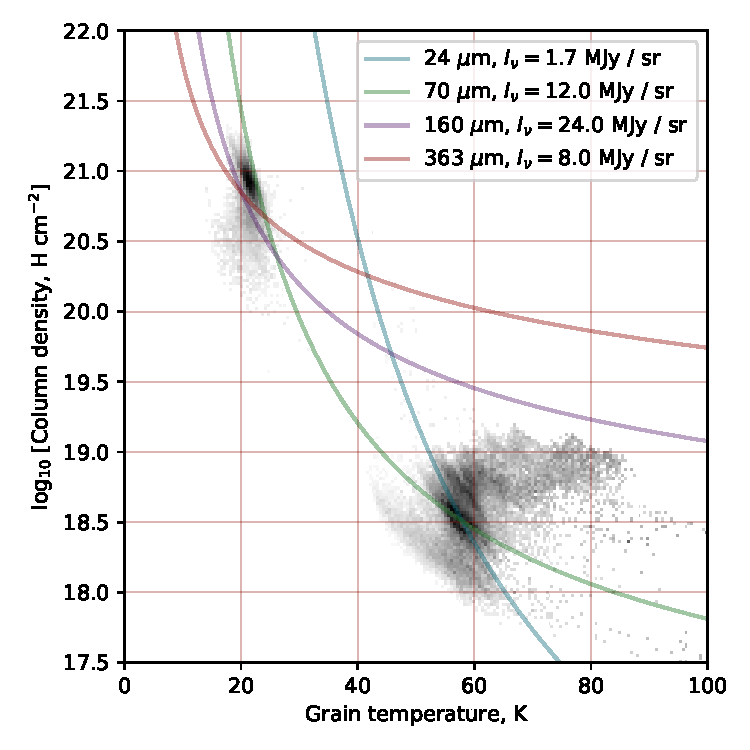
\includegraphics[width=\linewidth]{figs/sigma-ori-N-T-histogram}
  \caption{Joint distribution of dust temperature and gas column
    density. Gray-scale image shows the fraction of the emission at
    \SI{160}{\um} (cool component, upper-left) and \SI{24}{\um} (warm
    component, lower right) that is contributed by pixels with a given
    \((T, N)\) combination. Conversion from dust optical depth to
    hydrogen column density is carried out using the empirical
    calibration described in the text.}
  \label{fig:N-T-distro}
\end{figure}

\section{Conclusions}
\label{sec:conclusions}

\section*{Acknowledgements}

We are grateful for financial support provided by Dirección General de
Asuntos del Personal Académico, Universidad Nacional Autónoma de
México, through grant Programa de Apoyo a Proyectos de Investigación e
Inovación Tecnológica IN107019.  We thank Bo Reipurth for advice on
astronomical data archives.  This work is based in part on
observations made in the Observatorios de Canarias del IAC with the
Isaac Newton Telescope operated on the island of La Palma by the
Instituto de Astrofísica de Canarias in the Observatorio del Roque de
los Muchachos. 
% Based in part on observations made with the Isaac Newton Telescope
% under Director’s Discretionary Time of Spain’s Instituto de
% Astrofísica de Canarias.
This work is based in part on observations made with the Spitzer Space
Telescope, which is operated by the Jet Propulsion Laboratory,
California Institute of Technology under a contract with NASA.\@ This
work makes use of imagery from David Mittelman Astrophotography.

\bibliographystyle{mnras}
\bibliography{bowshocks-biblio}

% Don't change these lines
\bsp	% typesetting comment
\label{lastpage}
\end{document}

%%% Local Variables:
%%% mode: latex
%%% TeX-master: t
%%% End:
